
%% bare_jrnl_compsoc.tex
%% V1.3
%% 2007/01/11
%% by Michael Shell
%% See:
%% http://www.michaelshell.org/
%% for current contact information.
%%
%% This is a skeleton file demonstrating the use of IEEEtran.cls
%% (requires IEEEtran.cls version 1.7 or later) with an IEEE Computer
%% Society journal paper.
%%
%% Support sites:
%% http://www.michaelshell.org/tex/ieeetran/
%% http://www.ctan.org/tex-archive/macros/latex/contrib/IEEEtran/
%% and
%% http://www.ieee.org/

%%*************************************************************************
%% Legal Notice:
%% This code is offered as-is without any warranty either expressed or
%% implied; without even the implied warranty of MERCHANTABILITY or
%% FITNESS FOR A PARTICULAR PURPOSE! 
%% User assumes all risk.
%% In no event shall IEEE or any contributor to this code be liable for
%% any damages or losses, including, but not limited to, incidental,
%% consequential, or any other damages, resulting from the use or misuse
%% of any information contained here.
%%
%% All comments are the opinions of their respective authors and are not
%% necessarily endorsed by the IEEE.
%%
%% This work is distributed under the LaTeX Project Public License (LPPL)
%% ( http://www.latex-project.org/ ) version 1.3, and may be freely used,
%% distributed and modified. A copy of the LPPL, version 1.3, is included
%% in the base LaTeX documentation of all distributions of LaTeX released
%% 2003/12/01 or later.
%% Retain all contribution notices and credits.
%% ** Modified files should be clearly indicated as such, including  **
%% ** renaming them and changing author support contact information. **
%%
%% File list of work: IEEEtran.cls, IEEEtran_HOWTO.pdf, bare_adv.tex,
%%                    bare_conf.tex, bare_jrnl.tex, bare_jrnl_compsoc.tex
%%*************************************************************************

% *** Authors should verify (and, if needed, correct) their LaTeX system  ***
% *** with the testflow diagnostic prior to trusting their LaTeX platform ***
% *** with production work. IEEE's font choices can trigger bugs that do  ***
% *** not appear when using other class files.                            ***
% The testflow support page is at:
% http://www.michaelshell.org/tex/testflow/




% Note that the a4paper option is mainly intended so that authors in
% countries using A4 can easily print to A4 and see how their papers will
% look in print - the typesetting of the document will not typically be
% affected with changes in paper size (but the bottom and side margins will).
% Use the testflow package mentioned above to verify correct handling of
% both paper sizes by the user's LaTeX system.
%
% Also note that the "draftcls" or "draftclsnofoot", not "draft", option
% should be used if it is desired that the figures are to be displayed in
% draft mode.
%
% The Computer Society usually requires 10pt for submissions.
%
\documentclass[10pt,journal,cspaper,compsoc]{IEEEtran}
%
% If IEEEtran.cls has not been installed into the LaTeX system files,
% manually specify the path to it like:
% \documentclass[12pt,journal,compsoc]{../sty/IEEEtran}





% Some very useful LaTeX packages include:
% (uncomment the ones you want to load)


% *** MISC UTILITY PACKAGES ***
%
%\usepackage{ifpdf}
% Heiko Oberdiek's ifpdf.sty is very useful if you need conditional
% compilation based on whether the output is pdf or dvi.
% usage:
% \ifpdf
%   % pdf code
% \else
%   % dvi code
% \fi
% The latest version of ifpdf.sty can be obtained from:
% http://www.ctan.org/tex-archive/macros/latex/contrib/oberdiek/
% Also, note that IEEEtran.cls V1.7 and later provides a builtin
% \ifCLASSINFOpdf conditional that works the same way.
% When switching from latex to pdflatex and vice-versa, the compiler may
% have to be run twice to clear warning/error messages.






% *** CITATION PACKAGES ***
%
\ifCLASSOPTIONcompsoc
  % IEEE Computer Society needs nocompress option
  % requires cite.sty v4.0 or later (November 2003)
  % \usepackage[nocompress]{cite}
\else
  % normal IEEE
  % \usepackage{cite}
\fi
% cite.sty was written by Donald Arseneau
% V1.6 and later of IEEEtran pre-defines the format of the cite.sty package
% \cite{} output to follow that of IEEE. Loading the cite package will
% result in citation numbers being automatically sorted and properly
% "compressed/ranged". e.g., [1], [9], [2], [7], [5], [6] without using
% cite.sty will become [1], [2], [5]--[7], [9] using cite.sty. cite.sty's
% \cite will automatically add leading space, if needed. Use cite.sty's
% noadjust option (cite.sty V3.8 and later) if you want to turn this off.
% cite.sty is already installed on most LaTeX systems. Be sure and use
% version 4.0 (2003-05-27) and later if using hyperref.sty. cite.sty does
% not currently provide for hyperlinked citations.
% The latest version can be obtained at:
% http://www.ctan.org/tex-archive/macros/latex/contrib/cite/
% The documentation is contained in the cite.sty file itself.
%
% Note that some packages require special options to format as the Computer
% Society requires. In particular, Computer Society  papers do not use
% compressed citation ranges as is done in typical IEEE papers
% (e.g., [1]-[4]). Instead, they list every citation separately in order
% (e.g., [1], [2], [3], [4]). To get the latter we need to load the cite
% package with the nocompress option which is supported by cite.sty v4.0
% and later. Note also the use of a CLASSOPTION conditional provided by
% IEEEtran.cls V1.7 and later.





% *** GRAPHICS RELATED PACKAGES ***
%
\ifCLASSINFOpdf
  \usepackage[pdftex]{graphicx}
  % declare the path(s) where your graphic files are
   \graphicspath{{images/}}
  % and their extensions so you won't have to specify these with
  % every instance of \includegraphics
  \DeclareGraphicsExtensions{.pdf,.jpeg,.png}
\else
  % or other class option (dvipsone, dvipdf, if not using dvips). graphicx
  % will default to the driver specified in the system graphics.cfg if no
  % driver is specified.
  % \usepackage[dvips]{graphicx}
  % declare the path(s) where your graphic files are
  % \graphicspath{{../eps/}}
  % and their extensions so you won't have to specify these with
  % every instance of \includegraphics
  % \DeclareGraphicsExtensions{.eps}
\fi
% graphicx was written by David Carlisle and Sebastian Rahtz. It is
% required if you want graphics, photos, etc. graphicx.sty is already
% installed on most LaTeX systems. The latest version and documentation can
% be obtained at: 
% http://www.ctan.org/tex-archive/macros/latex/required/graphics/
% Another good source of documentation is "Using Imported Graphics in
% LaTeX2e" by Keith Reckdahl which can be found as epslatex.ps or
% epslatex.pdf at: http://www.ctan.org/tex-archive/info/
%
% latex, and pdflatex in dvi mode, support graphics in encapsulated
% postscript (.eps) format. pdflatex in pdf mode supports graphics
% in .pdf, .jpeg, .png and .mps (metapost) formats. Users should ensure
% that all non-photo figures use a vector format (.eps, .pdf, .mps) and
% not a bitmapped formats (.jpeg, .png). IEEE frowns on bitmapped formats
% which can result in "jaggedy"/blurry rendering of lines and letters as
% well as large increases in file sizes.
%
% You can find documentation about the pdfTeX application at:
% http://www.tug.org/applications/pdftex





% *** MATH PACKAGES ***
%
\usepackage[cmex10]{amsmath}
% A popular package from the American Mathematical Society that provides
% many useful and powerful commands for dealing with mathematics. If using
% it, be sure to load this package with the cmex10 option to ensure that
% only type 1 fonts will utilized at all point sizes. Without this option,
% it is possible that some math symbols, particularly those within
% footnotes, will be rendered in bitmap form which will result in a
% document that can not be IEEE Xplore compliant!
%
% Also, note that the amsmath package sets \interdisplaylinepenalty to 10000
% thus preventing page breaks from occurring within multiline equations. Use:
%\interdisplaylinepenalty=2500
% after loading amsmath to restore such page breaks as IEEEtran.cls normally
% does. amsmath.sty is already installed on most LaTeX systems. The latest
% version and documentation can be obtained at:
% http://www.ctan.org/tex-archive/macros/latex/required/amslatex/math/





% *** SPECIALIZED LIST PACKAGES ***
%
%\usepackage{algorithmic}
% algorithmic.sty was written by Peter Williams and Rogerio Brito.
% This package provides an algorithmic environment fo describing algorithms.
% You can use the algorithmic environment in-text or within a figure
% environment to provide for a floating algorithm. Do NOT use the algorithm
% floating environment provided by algorithm.sty (by the same authors) or
% algorithm2e.sty (by Christophe Fiorio) as IEEE does not use dedicated
% algorithm float types and packages that provide these will not provide
% correct IEEE style captions. The latest version and documentation of
% algorithmic.sty can be obtained at:
% http://www.ctan.org/tex-archive/macros/latex/contrib/algorithms/
% There is also a support site at:
% http://algorithms.berlios.de/index.html
% Also of interest may be the (relatively newer and more customizable)
% algorithmicx.sty package by Szasz Janos:
% http://www.ctan.org/tex-archive/macros/latex/contrib/algorithmicx/




% *** ALIGNMENT PACKAGES ***
%
%\usepackage{array}
% Frank Mittelbach's and David Carlisle's array.sty patches and improves
% the standard LaTeX2e array and tabular environments to provide better
% appearance and additional user controls. As the default LaTeX2e table
% generation code is lacking to the point of almost being broken with
% respect to the quality of the end results, all users are strongly
% advised to use an enhanced (at the very least that provided by array.sty)
% set of table tools. array.sty is already installed on most systems. The
% latest version and documentation can be obtained at:
% http://www.ctan.org/tex-archive/macros/latex/required/tools/


%\usepackage{mdwmath}
%\usepackage{mdwtab}
% Also highly recommended is Mark Wooding's extremely powerful MDW tools,
% especially mdwmath.sty and mdwtab.sty which are used to format equations
% and tables, respectively. The MDWtools set is already installed on most
% LaTeX systems. The lastest version and documentation is available at:
% http://www.ctan.org/tex-archive/macros/latex/contrib/mdwtools/


% IEEEtran contains the IEEEeqnarray family of commands that can be used to
% generate multiline equations as well as matrices, tables, etc., of high
% quality.


%\usepackage{eqparbox}
% Also of notable interest is Scott Pakin's eqparbox package for creating
% (automatically sized) equal width boxes - aka "natural width parboxes".
% Available at:
% http://www.ctan.org/tex-archive/macros/latex/contrib/eqparbox/





% *** SUBFIGURE PACKAGES ***
%\ifCLASSOPTIONcompsoc
%\usepackage[tight,normalsize,sf,SF]{subfigure}
%\else
%\usepackage[tight,footnotesize]{subfigure}
%\fi
% subfigure.sty was written by Steven Douglas Cochran. This package makes it
% easy to put subfigures in your figures. e.g., "Figure 1a and 1b". For IEEE
% work, it is a good idea to load it with the tight package option to reduce
% the amount of white space around the subfigures. Computer Society papers
% use a larger font and \sffamily font for their captions, hence the
% additional options needed under compsoc mode. subfigure.sty is already
% installed on most LaTeX systems. The latest version and documentation can
% be obtained at:
% http://www.ctan.org/tex-archive/obsolete/macros/latex/contrib/subfigure/
% subfigure.sty has been superceeded by subfig.sty.


%\ifCLASSOPTIONcompsoc
%  \usepackage[caption=false]{caption}
%  \usepackage[font=normalsize,labelfont=sf,textfont=sf]{subfig}
%\else
%  \usepackage[caption=false]{caption}
%  \usepackage[font=footnotesize]{subfig}
%\fi
% subfig.sty, also written by Steven Douglas Cochran, is the modern
% replacement for subfigure.sty. However, subfig.sty requires and
% automatically loads Axel Sommerfeldt's caption.sty which will override
% IEEEtran.cls handling of captions and this will result in nonIEEE style
% figure/table captions. To prevent this problem, be sure and preload
% caption.sty with its "caption=false" package option. This is will preserve
% IEEEtran.cls handing of captions. Version 1.3 (2005/06/28) and later 
% (recommended due to many improvements over 1.2) of subfig.sty supports
% the caption=false option directly:
%\ifCLASSOPTIONcompsoc
%  \usepackage[caption=false,font=normalsize,labelfont=sf,textfont=sf]{subfig}
%\else
%  \usepackage[caption=false,font=footnotesize]{subfig}
%\fi
%
% The latest version and documentation can be obtained at:
% http://www.ctan.org/tex-archive/macros/latex/contrib/subfig/
% The latest version and documentation of caption.sty can be obtained at:
% http://www.ctan.org/tex-archive/macros/latex/contrib/caption/




% *** FLOAT PACKAGES ***
%
%\usepackage{fixltx2e}
% fixltx2e, the successor to the earlier fix2col.sty, was written by
% Frank Mittelbach and David Carlisle. This package corrects a few problems
% in the LaTeX2e kernel, the most notable of which is that in current
% LaTeX2e releases, the ordering of single and double column floats is not
% guaranteed to be preserved. Thus, an unpatched LaTeX2e can allow a
% single column figure to be placed prior to an earlier double column
% figure. The latest version and documentation can be found at:
% http://www.ctan.org/tex-archive/macros/latex/base/



%\usepackage{stfloats}
% stfloats.sty was written by Sigitas Tolusis. This package gives LaTeX2e
% the ability to do double column floats at the bottom of the page as well
% as the top. (e.g., "\begin{figure*}[!b]" is not normally possible in
% LaTeX2e). It also provides a command:
%\fnbelowfloat
% to enable the placement of footnotes below bottom floats (the standard
% LaTeX2e kernel puts them above bottom floats). This is an invasive package
% which rewrites many portions of the LaTeX2e float routines. It may not work
% with other packages that modify the LaTeX2e float routines. The latest
% version and documentation can be obtained at:
% http://www.ctan.org/tex-archive/macros/latex/contrib/sttools/
% Documentation is contained in the stfloats.sty comments as well as in the
% presfull.pdf file. Do not use the stfloats baselinefloat ability as IEEE
% does not allow \baselineskip to stretch. Authors submitting work to the
% IEEE should note that IEEE rarely uses double column equations and
% that authors should try to avoid such use. Do not be tempted to use the
% cuted.sty or midfloat.sty packages (also by Sigitas Tolusis) as IEEE does
% not format its papers in such ways.




%\ifCLASSOPTIONcaptionsoff
%  \usepackage[nomarkers]{endfloat}
% \let\MYoriglatexcaption\caption
% \renewcommand{\caption}[2][\relax]{\MYoriglatexcaption[#2]{#2}}
%\fi
% endfloat.sty was written by James Darrell McCauley and Jeff Goldberg.
% This package may be useful when used in conjunction with IEEEtran.cls'
% captionsoff option. Some IEEE journals/societies require that submissions
% have lists of figures/tables at the end of the paper and that
% figures/tables without any captions are placed on a page by themselves at
% the end of the document. If needed, the draftcls IEEEtran class option or
% \CLASSINPUTbaselinestretch interface can be used to increase the line
% spacing as well. Be sure and use the nomarkers option of endfloat to
% prevent endfloat from "marking" where the figures would have been placed
% in the text. The two hack lines of code above are a slight modification of
% that suggested by in the endfloat docs (section 8.3.1) to ensure that
% the full captions always appear in the list of figures/tables - even if
% the user used the short optional argument of \caption[]{}.
% IEEE papers do not typically make use of \caption[]'s optional argument,
% so this should not be an issue. A similar trick can be used to disable
% captions of packages such as subfig.sty that lack options to turn off
% the subcaptions:
% For subfig.sty:
% \let\MYorigsubfloat\subfloat
% \renewcommand{\subfloat}[2][\relax]{\MYorigsubfloat[]{#2}}
% For subfigure.sty:
% \let\MYorigsubfigure\subfigure
% \renewcommand{\subfigure}[2][\relax]{\MYorigsubfigure[]{#2}}
% However, the above trick will not work if both optional arguments of
% the \subfloat/subfig command are used. Furthermore, there needs to be a
% description of each subfigure *somewhere* and endfloat does not add
% subfigure captions to its list of figures. Thus, the best approach is to
% avoid the use of subfigure captions (many IEEE journals avoid them anyway)
% and instead reference/explain all the subfigures within the main caption.
% The latest version of endfloat.sty and its documentation can obtained at:
% http://www.ctan.org/tex-archive/macros/latex/contrib/endfloat/
%
% The IEEEtran \ifCLASSOPTIONcaptionsoff conditional can also be used
% later in the document, say, to conditionally put the References on a 
% page by themselves.




% *** PDF, URL AND HYPERLINK PACKAGES ***
%
\usepackage{url}
% url.sty was written by Donald Arseneau. It provides better support for
% handling and breaking URLs. url.sty is already installed on most LaTeX
% systems. The latest version can be obtained at:
% http://www.ctan.org/tex-archive/macros/latex/contrib/misc/
% Read the url.sty source comments for usage information. Basically,
% \url{my_url_here}.



%\usepackage{natbib}

% *** Do not adjust lengths that control margins, column widths, etc. ***
% *** Do not use packages that alter fonts (such as pslatex).         ***
% There should be no need to do such things with IEEEtran.cls V1.6 and later.
% (Unless specifically asked to do so by the journal or conference you plan
% to submit to, of course. )


% correct bad hyphenation here
\hyphenation{op-tical net-works semi-conduc-tor}


\begin{document}
%
% paper title
% can use linebreaks \\ within to get better formatting as desired
\title{Common Angle Plots as perception-true visualizations of categorical associations}
%
%
% author names and IEEE memberships
% note positions of commas and nonbreaking spaces ( ~ ) LaTeX will not break
% a structure at a ~ so this keeps an author's name from being broken across
% two lines.
% use \thanks{} to gain access to the first footnote area
% a separate \thanks must be used for each paragraph as LaTeX2e's \thanks
% was not built to handle multiple paragraphs
%
%
%\IEEEcompsocitemizethanks is a special \thanks that produces the bulleted
% lists the Computer Society journals use for "first footnote" author
% affiliations. Use \IEEEcompsocthanksitem which works much like \item
% for each affiliation group. When not in compsoc mode,
% \IEEEcompsocitemizethanks becomes like \thanks and
% \IEEEcompsocthanksitem becomes a line break with idention. This
% facilitates dual compilation, although admittedly the differences in the
% desired content of \author between the different types of papers makes a
% one-size-fits-all approach a daunting prospect. For instance, compsoc 
% journal papers have the author affiliations above the "Manuscript
% received ..."  text while in non-compsoc journals this is reversed. Sigh.

%
%\author{Heike~Hofmann,~\IEEEmembership{Member,~IEEE,}
%        and~Marie~Vendettuoli% <-this % stops a space
%\thanks{H. Hofmann, faculty member in the Department
%of Statistics, Iowa State University, Ames,
%IA, 50014 USA e-mail: hofmann@iastate.edu.}% <-this % stops a space
%\thanks{M. Vendettuoli, Graduate Student in the HCI and BCB programs at Iowa State University and member of the Statistics Section of USDA APHIS Center for Veterinary Biologics in Ames, IA 50014.}% <-this % stops a space
%\thanks{Manuscript received Nov 1, 2012; revised Mar , 2013}}

\author{Heike~Hofmann,~\IEEEmembership{Member,~IEEE,}
        and~Marie~Vendettuoli%
%,~\IEEEmembership{Fellow,~OSA,}
%        and~Jane~Doe,~\IEEEmembership{Life~Fellow,~IEEE}% <-this % stops a space
\IEEEcompsocitemizethanks{\IEEEcompsocthanksitem H. Hofmann is faculty with the Department
of Statistics, \protect\\
Iowa State University, Ames,
IA, 50014.\protect\\
% note need leading \protect in front of \\ to get a newline within \thanks as
% \\ is fragile and will error, could use \hfil\break instead.
E-mail: hofmann@iastate.edu
\IEEEcompsocthanksitem M. Vendettuoli is graduate student \protect\\ HCI and BCB programs, 
 Iowa State University \protect\\
and member of the Statistics Section, USDA APHIS CVB \protect\\ Ames, IA 50014}% <-this % stops a space
\thanks{}}

% note the % following the last \IEEEmembership and also \thanks - 
% these prevent an unwanted space from occurring between the last author name
% and the end of the author line. i.e., if you had this:
% 
% \author{....lastname \thanks{...} \thanks{...} }
%                     ^------------^------------^----Do not want these spaces!
%
% a space would be appended to the last name and could cause every name on that
% line to be shifted left slightly. This is one of those "LaTeX things". For
% instance, "\textbf{A} \textbf{B}" will typeset as "A B" not "AB". To get
% "AB" then you have to do: "\textbf{A}\textbf{B}"
% \thanks is no different in this regard, so shield the last } of each \thanks
% that ends a line with a % and do not let a space in before the next \thanks.
% Spaces after \IEEEmembership other than the last one are OK (and needed) as
% you are supposed to have spaces between the names. For what it is worth,
% this is a minor point as most people would not even notice if the said evil
% space somehow managed to creep in.



% The paper headers
\markboth{Journal of \LaTeX\ Class Files,~Vol.~6, No.~1, January~2007}%
{Shell \MakeLowercase{\textit{et al.}}: Bare Demo of IEEEtran.cls for Computer Society Journals}
% The only time the second header will appear is for the odd numbered pages
% after the title page when using the twoside option.
% 
% *** Note that you probably will NOT want to include the author's ***
% *** name in the headers of peer review papers.                   ***
% You can use \ifCLASSOPTIONpeerreview for conditional compilation here if
% you desire.



% The publisher's ID mark at the bottom of the page is less important with
% Computer Society journal papers as those publications place the marks
% outside of the main text columns and, therefore, unlike regular IEEE
% journals, the available text space is not reduced by their presence.
% If you want to put a publisher's ID mark on the page you can do it like
% this:
%\IEEEpubid{0000--0000/00\$00.00~\copyright~2007 IEEE}
% or like this to get the Computer Society new two part style.
%\IEEEpubid{\makebox[\columnwidth]{\hfill 0000--0000/00/\$00.00~\copyright~2007 IEEE}%
%\hspace{\columnsep}\makebox[\columnwidth]{Published by the IEEE Computer Society\hfill}}
% Remember, if you use this you must call \IEEEpubidadjcol in the second
% column for its text to clear the IEEEpubid mark (Computer Society jorunal
% papers don't need this extra clearance.)




% for Computer Society papers, we must declare the abstract and index terms
% PRIOR to the title within the \IEEEcompsoctitleabstractindextext IEEEtran
% command as these need to go into the title area created by \maketitle.
\IEEEcompsoctitleabstractindextext{%
\begin{abstract}
%\boldmath

Visualizations are great tools of communications - they summarize findings and quickly convey main messages to our audience. As designers of charts we have to make sure that information is shown with a minimum of distortion. We have to also consider illusions and other perceptual  limitations of our audience. In this paper we discuss  the effect and strength of the  line width illusion,  a M\"uller-Lyer type illusion, on designs related to displaying associations between categorical variables. Parallel sets and hammock plots are both affected by line width illusions. We  introduce the common-angle plot as an alternative method for displaying categorical data in a manner that minimizes the effect from perceptual illusions.
Finally, we present results from user studies as evidence that common angle charts resolve  problems with the line width illusion.
\end{abstract}
% IEEEtran.cls defaults to using nonbold math in the Abstract.
% This preserves the distinction between vectors and scalars. However,
% if the journal you are submitting to favors bold math in the abstract,
% then you can use LaTeX's standard command \boldmath at the very start
% of the abstract to achieve this. Many IEEE journals frown on math
% in the abstract anyway. In particular, the Computer Society does
% not want either math or citations to appear in the abstract.

% Note that keywords are not normally used for peer review papers.
\begin{IEEEkeywords}
Linewidth illusion, Data Visualization, High-dimensional Displays, Parallel Sets, Hammock Plots, M\"uller-Lyer Illusion.
\end{IEEEkeywords}
}


% make the title area
\maketitle


% To allow for easy dual compilation without having to reenter the
% abstract/keywords data, the \IEEEcompsoctitleabstractindextext text will
% not be used in maketitle, but will appear (i.e., to be "transported")
% here as \IEEEdisplaynotcompsoctitleabstractindextext when compsoc mode
% is not selected <OR> if conference mode is selected - because compsoc
% conference papers position the abstract like regular (non-compsoc)
% papers do!
\IEEEdisplaynotcompsoctitleabstractindextext
% \IEEEdisplaynotcompsoctitleabstractindextext has no effect when using
% compsoc under a non-conference mode.


% For peer review papers, you can put extra information on the cover
% page as needed:
% \ifCLASSOPTIONpeerreview
% \begin{center} \bfseries EDICS Category: 3-BBND \end{center}
% \fi
%
% For peerreview papers, this IEEEtran command inserts a page break and
% creates the second title. It will be ignored for other modes.
\IEEEpeerreviewmaketitle



%\section{Introduction}
% Computer Society journal papers do something a tad strange with the very
% first section heading (almost always called "Introduction"). They place it
% ABOVE the main text! IEEEtran.cls currently does not do this for you.
% However, You can achieve this effect by making LaTeX jump through some
% hoops via something like:
%
%\ifCLASSOPTIONcompsoc
%  \noindent\raisebox{2\baselineskip}[0pt][0pt]%
%  {\parbox{\columnwidth}{\section{Introduction}\label{sec:introduction}%
%  \global\everypar=\everypar}}%
%  \vspace{-1\baselineskip}\vspace{-\parskip}\par
%\else
%  \section{Introduction}\label{sec:introduction}\par
%\fi
%
% Admittedly, this is a hack and may well be fragile, but seems to do the
% trick for me. Note the need to keep any \label that may be used right
% after \section in the above as the hack puts \section within a raised box.



% The very first letter is a 2 line initial drop letter followed
% by the rest of the first word in caps (small caps for compsoc).
% 
% form to use if the first word consists of a single letter:
% \IEEEPARstart{A}{demo} file is ....
% 
% form to use if you need the single drop letter followed by
% normal text (unknown if ever used by IEEE):
% \IEEEPARstart{A}{}demo file is ....
% 
% Some journals put the first two words in caps:
% \IEEEPARstart{T}{his demo} file is ....
% 
% Here we have the typical use of a "T" for an initial drop letter
% and "HIS" in caps to complete the first word.
%\IEEEPARstart{T}{his} demo file is intended to serve as a ``starter file''
%for IEEE Computer Society journal papers produced under \LaTeX\ using
%IEEEtran.cls version 1.7 and later.
% You must have at least 2 lines in the paragraph with the drop letter
% (should never be an issue)
%I wish you the best of success.
%
%\hfill mds
 
% !TEX root = bare_jrnl_compsoc.tex


\section{Introduction}
% The very first letter is a 2 line initial drop letter followed
% by the rest of the first word in caps.
% 
% form to use if the first word consists of a single letter:
% \IEEEPARstart{A}{demo} file is ....
% 
% form to use if you need the single drop letter followed by
% normal text (unknown if ever used by IEEE):
% \IEEEPARstart{A}{}demo file is ....
% 
% Some journals put the first two words in caps:
% \IEEEPARstart{T}{his demo} file is ....
% 
% Here we have the typical use of a "T" for an initial drop letter
% and "HIS" in caps to complete the first word.
\IEEEPARstart{A}{ well-designed} graph is a powerful tool 
that transends barriers of language to
communicate complex concepts from author to audience. It becomes a 
problem if readers are unable to easily extract the main message, especially
when distortion is encoded. The source of a distortion may be due to 
intrinsic deformities in the graph or simply the perceptual limitations of
the audience. Examples include Tufte's \emph{Lie-Factor} \cite[p. 57--69]{tufte} in which the proportion of the physical space occupied by the graphic is 
inconsistent with underlying data; calculated ratio (of proportions) less than one indicate 
underrepresentation. Another example is the M\"{u}ller-Lyer family of illusions such as the sine wave, where viewers perceive extents at the curves to be of different height than in the straight regions even though all regions were of the same height \cite{day:1991}.

Regardless of the cause of distortion, the graph author has a duty to create visualizations that
 allows readers to extract an accurate interpretation of the underlying data. The \emph{Lie-Factor}
provides a quantitative method to evaluate distortion due to graph deformities. In order to ascertain the
impact of distortion due to perceptual limits, usability studies provide empirical evidence supporting 
underlying metaphorical models, both known and unpredicted.  




Parallel sets (parsets)  \cite{kosara:2006}, a graphical method  for visualizing multivariate categorical data, presents a case of unspecified distortion due to perceptual limits . Since initial publication, parsets have spread to mass media outlets  \cite{eagereyes, bostock:2012, bbc:2009}, multiple technical implementations \cite{eagereyes, d3, davies} and is a reputable resource for further academic work (\cite{kosara:2006} has 70 citations per Google scholar). While retaining the %independent 
ability to visualize a large number of dimensions simultaneously that is the parallel coordinates' hallmark trade, parsets introduce the frequency scale that is a well-known feature of other categorical displays such as barcharts or mosaic plots \cite{hartigan:1981, friendly:1992, hofmann:2000, theus:1997}.
% Initially, frequencies of categories  were displayed as stacked boxes; in  later versions of parallel sets the boxes are reduced to simple lines \cite{parsetredesign}. Various implementations of parallel sets exist besides the original Java version of Eagereyes \cite{eagereyes}, e.g.  J Davies introduced a d3 \cite{d3} version in  \cite{davies}.  


\begin{figure}[hbtp]
\centering
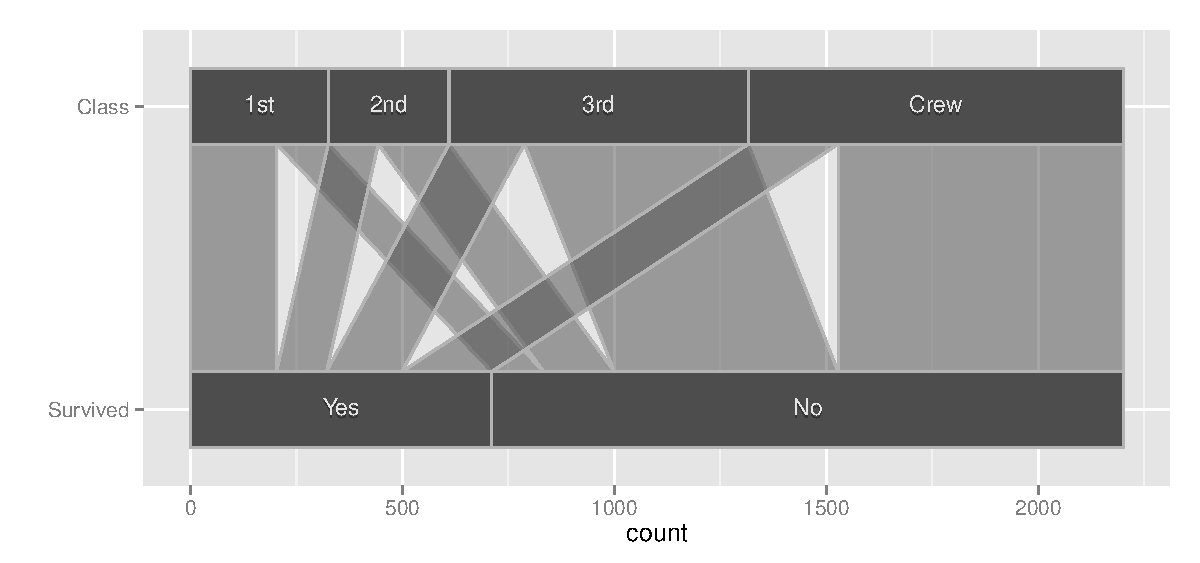
\includegraphics[width=.9\linewidth]{images/parset-titanic}
\caption{\label{question1a} Parallel sets plot showing the relationship between survival of the sinking of the HMS Titanic and class membership. }
\end{figure}
%XXX Description of parallel sets - and example


%%XXX PS and line-width illusion
Figure \ref{question1a} gives an example for a two dimensional parallel sets plot investigating the relationship between class status and survival on board the HMS Titanic  \cite{dawson:1995}. Class status is recorded as either crew member or passengers in  first, second, or third class.  The top bar in figure \ref{question1a} shows the  variable Class. The bottom bar shows survival  as yes and no. Between the bars lines are drawn to visualize the relationship between class membership and  survival. 
  Based on the number of survivor and non survivors
  these bands are drawn from each class, and their (horizontal) width is proportional to the number of people they represent. A reasonable task would be to order levels of the variable `class' by number of survivors. However, when study participants were asked to perform this task, only $12.5\%$ respondants 
selected the correct order \ref{raw}.

\begin{table}
\begin{center}
\begin{tabular}{rrrrr}
& Crew & 1st & 2nd & 3rd \\ \hline
Survivors & 212 & 203 & 118 & 178\\
Non-Survivors & 673 & 122 & 167 &  528  
\end{tabular}
\caption{Correct ordering of variable Class is: crew, first class, third class, followed by second class. }
\end{center}
\end{table}
We believe that readers view parsets they are subject to the \emph{line width illusion}, a perceptual distortion that we describe and quantify in this paper. We also propose and test \emph{common angle plots}, an alternative graphing method for visualizing multivariate categorical is not subject to the \emph{line width illusion}.
%XXX PS and line-width illusion


%
% You must have at least 2 lines in the paragraph with the drop letter
% (should never be an issue)

\section{Line width illusion}




\begin{figure}
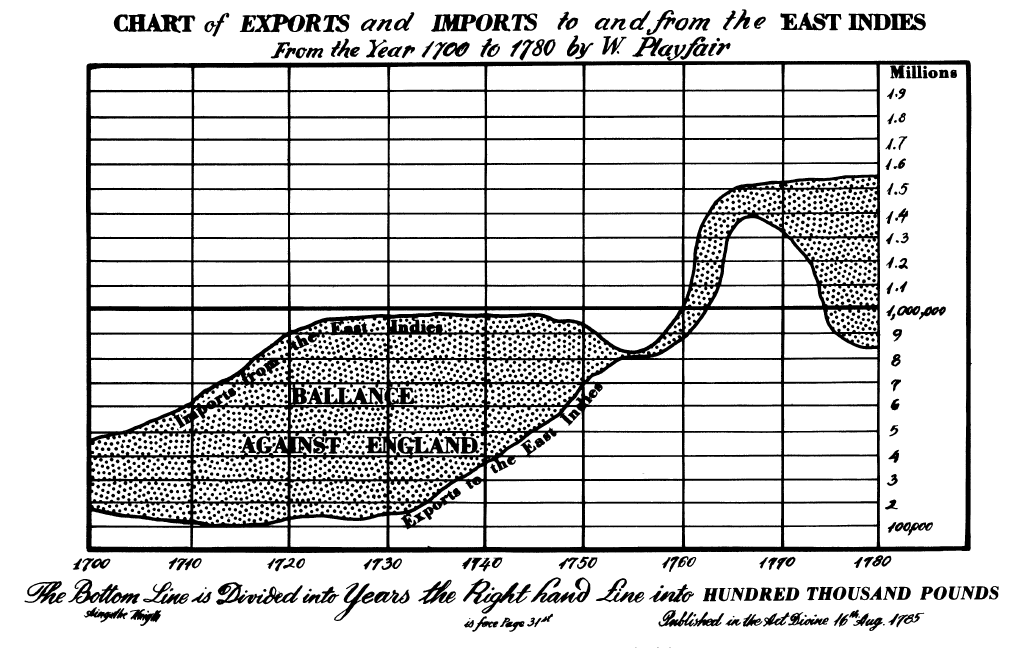
\includegraphics[width=.9\linewidth]{images/playfair_east_indies_gross}
\caption{\label{playfair}
Playfair's chart from the Commercial and Political Atlas (1786) showing the balance of trade between England and the East Indies.  In which years was the difference between imports and exports the highest? }
\end{figure}
An example of the  {\it line width illusion} is displayed in  figure  \ref{playfair}. This chart displays the balance of trade between England and the East Indies as shown by William Playfair in his Commercial and Political Atlas, 1786 \cite{playfair, playfair2}.  One purpose of this chart is to demonstrate the difference between imports and exports in a particular year and its pattern over that time frame. The difference in exports and imports is encoded as the vertical difference between the lines. When observers are asked to sketch out the difference between exports and imports  \cite{cleveland:1984}, they very often  miss the steep rise in the difference between the lines in the years between about 1755 and 1765. Figure \ref{playfair2} shows the  actual difference between imports and exports. 



\begin{figure}
\centering
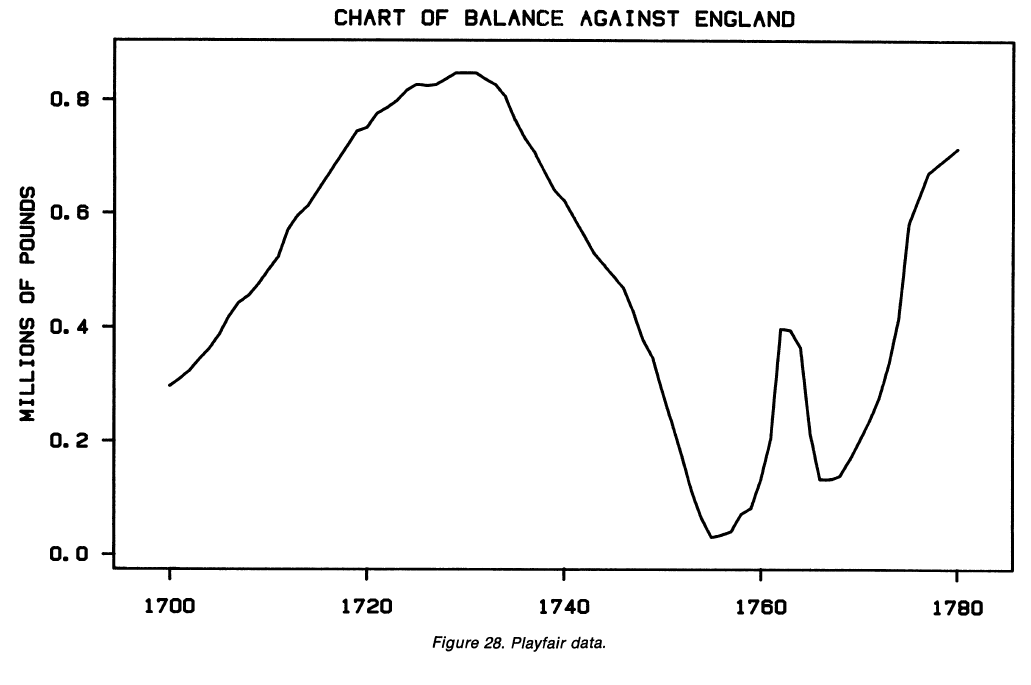
\includegraphics[width=.8\linewidth, height=.4\linewidth]{images/playfair_differenz_cleveland}
\caption{\label{playfair2}
Difference between exports and imports from England to and from the East Indies in the 18th century -- the steep rise in the difference around 1760  comes as a surprise to many viewers of the raw data in figure \ref{playfair}.  }
\end{figure}


This phenomenon  is known and widely discussed in statistical graphics literature \cite{cleveland:1984, tufte, wainer:2000, robbins:2005}. It  is due to our  tendency to assess distance between curves as the minimal (orthogonal) distance rather than the  vertical distance -- see sketch \ref{fig:linewidth} for a visual representation of both.


In the perception literature, this phenomenon is known as part of a group of geometrical optical misperceptions of a context-sensitive nature classified as M\"uller-Lyer illusions \cite{day:1991}. Interestingly, there seems to be a general agreement that this illusion exists, but a quantification of it is curiously absent from literature. 

The type of chart as shown in figure~\ref{playfair} proposed by Playfair is shown quite commonly, particular in election years -- where these kind of charts are used to enable comparisons of support for several candidates, the recommendation from literature is to avoid charts in which the audience is asked to do visual subtractions, and show these differences directly.

\subsection{Strength of  line width illusion}\label{distortion}

%The difference between perceived and actual line width 
When visually evaluating lines of thickness greater than one, the line width illusion applies, only now the {\it edges} of a single line  take on the role of the separate curves. %in the parallel sets 
As above, there is a strong preference of evaluating the width of lines orthogonal to their slopes as opposed to horizontally (see figure \ref{fig:linewidth})  needed for a correct  evaluation of parsets-style displays.

Orthogonal $w_o$ and horizontal $w_h$ line widths are related -- the orthogonal line width depends on the angle (or, equivalently, the slope) of the line:
\begin{equation}\label{adjust}
w_o = w_h \sin \theta,
\end{equation}
where $\theta$ is the angle of the line with respect to the horizontal line.

\begin{figure}[htbp]
\begin{center}
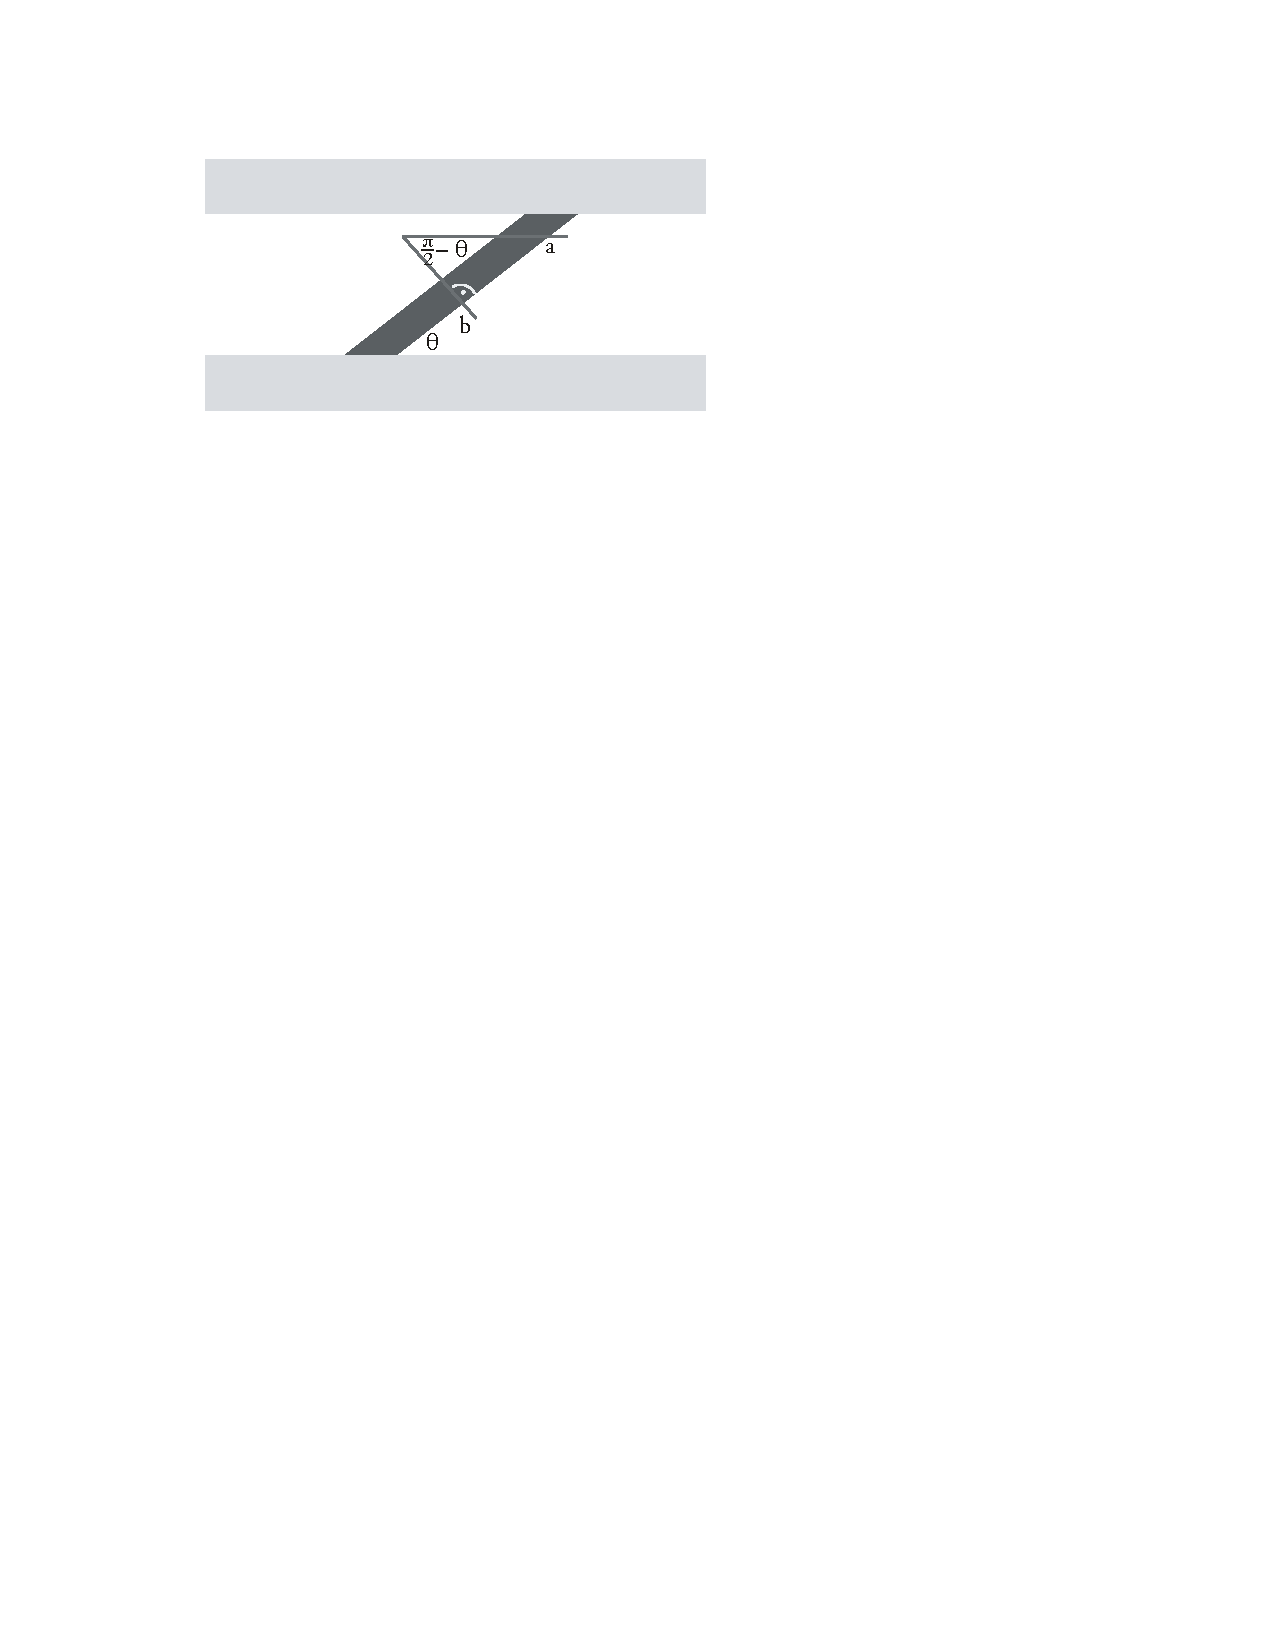
\includegraphics[width=0.6\linewidth]{images/linewidth}
\end{center}
\caption{\label{fig:linewidth}Sketch of line width assessments: (a) is showing  horizontal width, (b) shows  width orthogonal to the slope. Survey results in section \ref{results}  indicate that observers associate line width more with  orthogonal width (b) than horizontal width (a).}
\end{figure}



%XXX aspect ratio


\begin{figure*}[htbp]
\begin{center}
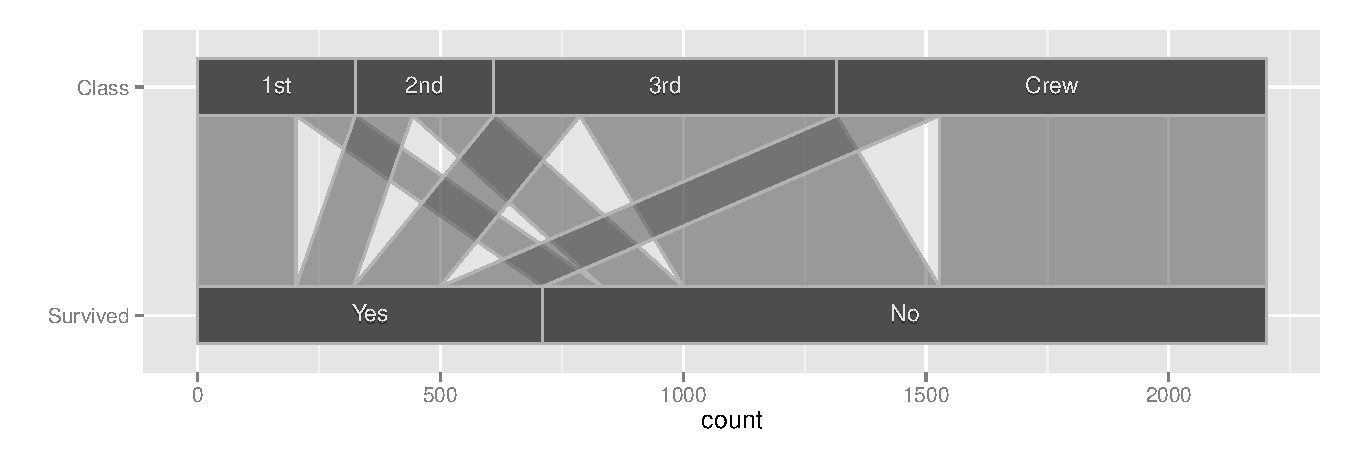
\includegraphics[height=1.5in]{images/aspect31-titanic.pdf}
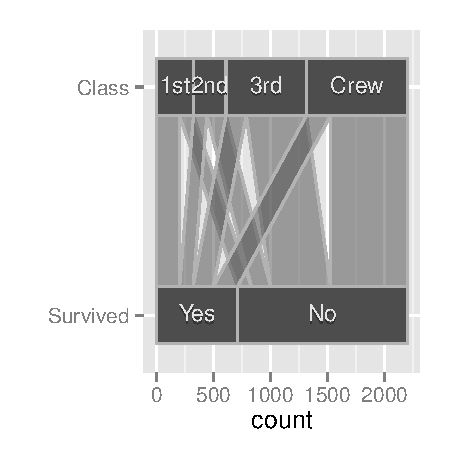
\includegraphics[height=1.5in]{images/aspect33-titanic.pdf}
\end{center}
\caption{\label{fig:aspect}Parallel sets plots of survival on the Titanic by class. Different aspect ratios  seemingly change the thickness of line segments, compare e.g. number of survivors in 3rd class and in the crew. }
\end{figure*}



The perceived slope of a line very much depends on the aspect ratio of the corresponding plot -- changing the height to width ratio of a display  will change our perception of the corresponding line widths, if they are not adjusted for the slope \cite{cleveland:1984}. This finding is not new, but its strength on our perception is surprising, as can be seen in the example of  figure \ref{fig:aspect}.  Again, survival and class membership on the Titanic is shown; the same parallel sets plot is shown twice in this figure, but with very different aspect ratios: in the  plot on the left the number of surviving 3rd class passengers seems to be about twice as big as the number of survivors among crew members, whereas in the plot on the right the lines have about equal (orthogonal) width. Obviously, this is not due to a change in numbers.

For parsets-style displays, the audience has {\it area of the line segment} an alternate visual cue when evaluating frequencies. Because height (or width for a rotated display) of  line segments is constant across the display, the width of a particular  segment is proportional to its area. We can therefore employ area comparisons as a proxy or to augment line width evaluations. 
However, existing literature suggests that this method of comparison is particularly  prone to errors in two scenarios commonly seen in parallel sets: (1) extreme aspect ratios of the rectangular shape \cite{heer:2010} %occupied by thick line segments 
and (2) when comparing rectangles rotated relative to each other \cite{kong:2010}. 
This incorrect perception and comparison of areas distorts the message readers discern from the graph. %additional contextual evidence that reinforce and strengthen distortion introduced by the line width illusion.


% needed in second column of first page if using \IEEEpubid
%\IEEEpubidadjcol
\section{Related work}
%XXX Description of hammock plots and example

Hammock plots, introduced by M Schonlau in \cite{schonlau:2003}, provide an alternative to parallel sets that is adjusted for the line width illusion. This is done by  adjusting the --horizontal-- line width by  a factor of $\sin \theta$, as discussed in equation (\ref{adjust}). This adjustment makes the perceived --orthogonal-- line width to be proportional to the number of observations it represents. 
 Figure \ref{hammock} shows an example of a four dimensional hammock plot of the Titanic data. From top to bottom Class, Gender, Survival, and again Class are shown. 
\begin{figure}
%cols <- c(brewer.pal(name="Blues", 6)[-c(1,2)], rev(brewer.pal(name="Oranges", 3)[-1]), rev(brewer.pal(name="Greens",3)[-1]))
%ggparallel(names(titanic)[c(1,4,2,1)], order=c(0,1,1,0), method="hammock", ratio=.25, text.angle=0, titanic, weight="Freq") +
%  scale_fill_manual(values=cols, guide="none") +
%  scale_colour_manual(values=cols, guide="none") + coord_flip() 
%ggsave("hammock-titanic.pdf", width=6, height=8)
\centering
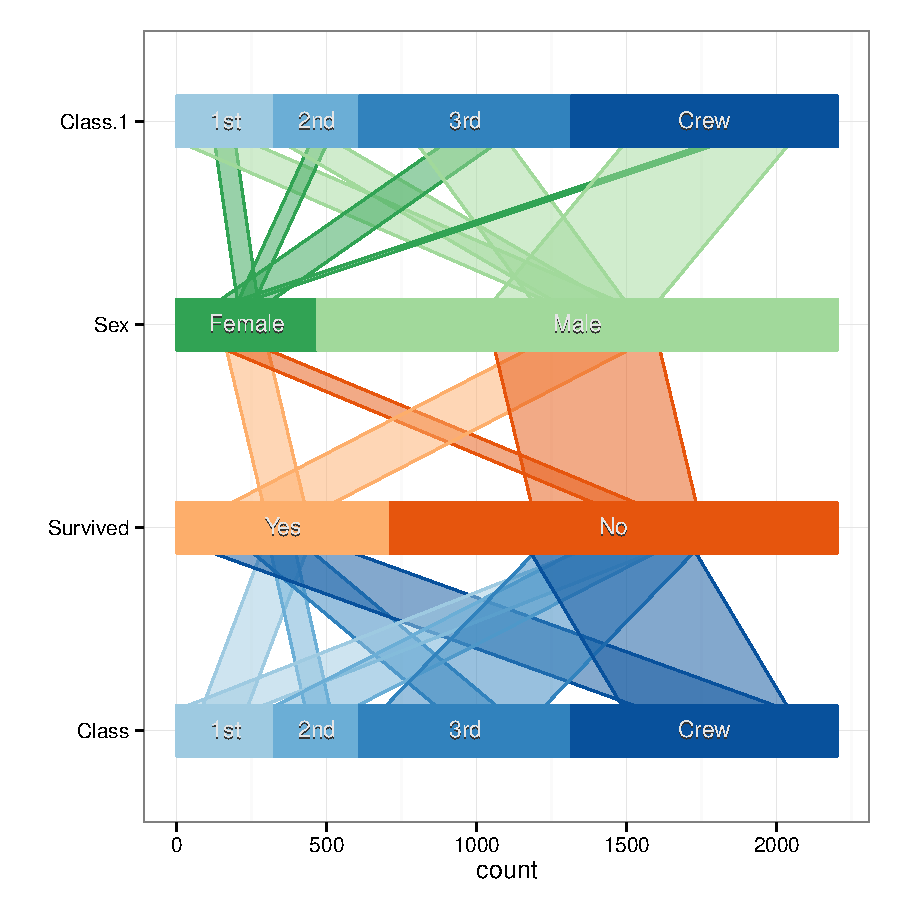
\includegraphics[width=\linewidth]{images/hammock-titanic}
\caption{\label{hammock} Hammock plot of the relationship between Class and Survival on the Titanic. }
\end{figure}

Similarly to the parallel sets plot, the bars are divided according to class membership numbers.  Lines connect categories between neighboring variables, orthogonal line widths are representing the number of individuals in each combination. Unlike the parallel sets, the lines start from the middle of the bin and connect to the middle of the other variable's bins. 

The graph shows that barely any women were in the crew, while male crew members make up the second largest contingent overall. Overall a few more men survived than women. Proportionally the situation is much different -- a much higher percentage of women survived than men. While more first class passengers survived than not, the  survival chances of second class passengers were about fifty-fifty. For third class passengers and crew members fewer members did  survive than not. 

As the adjustment of line widths is made with respect to the angle $\theta$, which itself depends on the aspect ratio of a plot, we need complete control over these properties of the plotting device when constructing hammock plots  -- in our implementation (see below for details) we have dealt with this issue by fixing the aspect ratio. This is problematic in some situations, where the rendering has to be done without knowledge of the plotting device. 

\subsection{Reverse linewidth}
A problem that arises in evaluating hammock plots is that if an observer focuses on horizontal line width  the plots suffer from a {\it reverse line width illusion}:  judging the number of survivors by class in figure \ref{hammock} based on horizontal line width  results in an ordering of (largest to smallest) Crew, 3rd, 1st, and 2nd -- which is not correct either. %Using horizontal width is inviting, since the lines are centered around the middle of a level, im
Because the lines are centered around the middle of each level, a contextual coordinate system is imposed that encourages comparisons of horizontal width. However, horizontal width alone is not proportional to underlying data. 

[[ If only h-width is considered, the graph has a lie factor; can we quantify this amount in terms of theta? ]]
%
%\section{Overview}
%From previous work \cite{cleveland:1984, tufte, wainer:2000, robbins:2005, heer:2010, kong:2010}, we may conclude that numerically accurate representations of data
%are subject to distortion due to perceptual limitations. In particular,
%the width of a single line of some thickness or the distance between two lines of minimal thickness is 
%subject to the \emph{line width illusion} even though the depiction is numerically sound.
% Furthermore, design choices during implementation \cite{schonlau:2003} may
%reduce the impact of such limitations.
%%

\section{Common angles}


\subsection{Construction}


\begin{figure}[htbp] %  figure placement: here, top, bottom, or page
%ggparallel(names(titanic)[c(1,4,2,1)], order=c(0,1,1,0), titanic, weight="Freq", text.angle=0) + 
%  scale_fill_manual(values=cols, guide="none") +
%  scale_colour_manual(values=cols, guide="none") + coord_flip() 
%ggsave("ca-titanic.pdf", width=6, height=6)
   \centering
   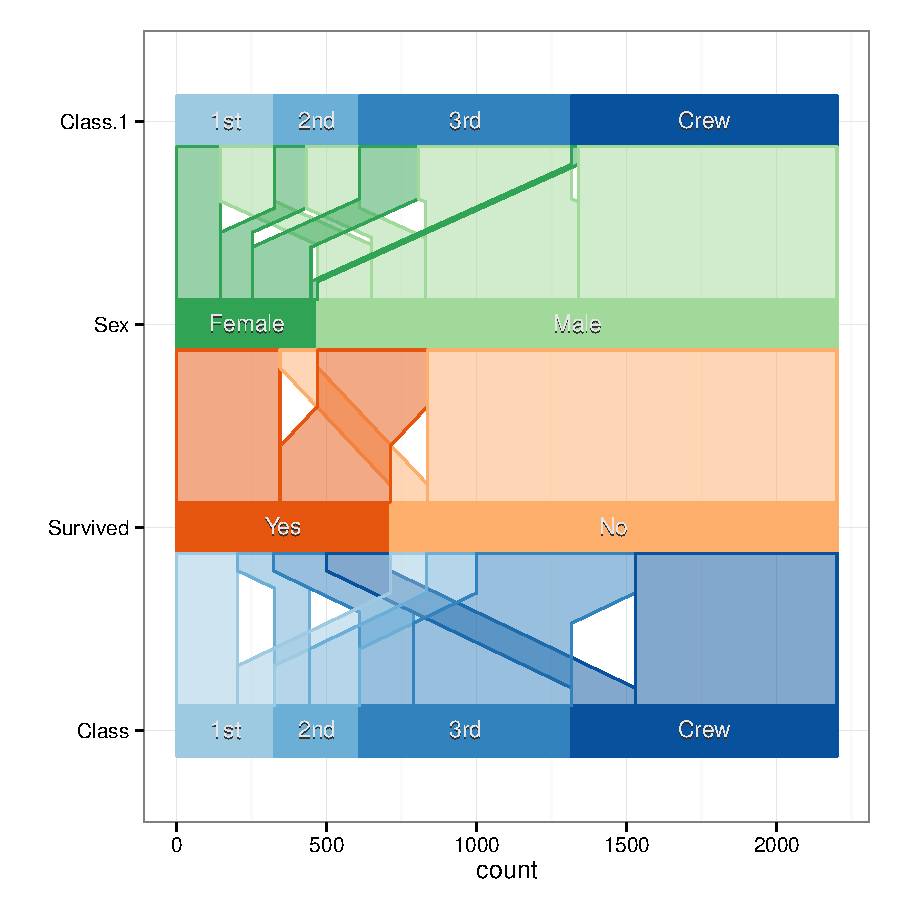
\includegraphics[width=\linewidth]{images/ca-titanic} 
   \caption{ \label{fig:ca-titanic} Common angle plot of the Titanic data. }
  \end{figure}

Figure \ref{fig:ca-titanic} shows a common angle plot of the same data as the hammock plot.

As in the previously discussed display types ribbons are drawn between categories with widths  that are proportional to  the number of records they represent.

In order to ensure that  widths of all bands are  comparable without any distortion, their slopes  are artificially made the same in the following manner: 
assuming a vertical display as shown in figure \ref{fig:ca-titanic}, we modify  the connecting bands between  categories from a straight band  to a combination of a vertical  segment, a  segment under a pre-specified angle $\theta$, followed by another vertical  segment.  
The pre-specified angle $\theta$ (between the line and the vertical band) is given as --at most-- the angle of the longest connecting line between two categories of neighboring variables. 
This makes the width of ribbons  comparable without being affected by the distortion, as all ribbons are sharing at least one segment under the same angle. 


\section{Usability Testing}
\subsection{Test}

To determine the effectiveness of the common angle plot, we conducted a user experiment in form of a survey asking participants to provide responses regarding the structure in two data sets with predominantly categorical variables.
For each data set, participants were asked to provide responses for three tasks:

Task I: simple comparison task, chosen to be unaffected by any illusion. Performance on this task should be comparable across the designs
Task II: comparison, affected by the line width illusion or its reverse. 
Task II: ordering task comprised of multiple comparisons, some of which are affected by either illusion.
  
Each participant was exposed to two of the three types of displays, one for all three tasks related to the same data set.
 
This resulted in six different survey administrations, with a crossover design as shown in Table \ref{tab:designs} that allows us to compare designs across different questions and data sets, and  simultaneously adjust for individuals' different skill sets.

\begin{table}[htbp]
\centering
\begin{tabular}{rrrrrrr}
Titanic Data & PS & CA & Ham & PS & CA & Ham \\ 
Pathway & CA & PS & PS & Ham & Ham & CA \\ \hline
\#responses &  8 (9) &  6 (7) &  8 (9) &  6 (7) & 10 (11) & 8 (8)\\ 
\end{tabular}
\caption{\label{tab:designs} Overview of study design and participation numbers. The number in parenthesis indicates the number of participants completing the first block, but not the second.}
\end{table}


\subsection{Results}

Answers for each question on the survey were assessed for correctness, and coded in binary variables of 1s and 0s, which we use to investigate performance of different designs. 

%In a first model, $M1$, we are only interested in the overall difference in performance between designs. We can express this as a model of the form
%\begin{equation}\label{model1}[M1]
%\quad\quad g(P(y_i=1)) = \mu + d_{j(i)} + u_{k(i)} + \varepsilon_i \quad\quad
%\end{equation}
%where $P(y_i=1)$ is the probability that the $i$th response is correct, for $i = 1, ..., n$. $g(.)$ is the transformation (link function) of the response. Here, we make use of the logit link, i.e.
%\begin{eqnarray*}
%g(P(y_i=1)) &=& \text{logit } P(y_i=1) = \\
%&=& \log P(y_i=1) - \log P(y_i=0).
%\end{eqnarray*}
%$d_{j(i)}$ is the parameter measuring the effect of design $j$ ($j = C, H, P$ for \underline{C}ommon Angle, \underline{H}ammock plot, and \underline{P}arallel sets plot), $u_{k(i)}$ is the effect of participant's $k$ individual skills in evaluating these plots, $k \in \{1, ..., 52\}$. The assumption is that skills are independent and normally distributed with an expected value of zero and a variance of $\sigma_u^2$.
%$\varepsilon_i$ is, similarly to a regular linear model, assumed to be independently distributed according to a normal distribution with mean of zero and variance $\sigma^2$.



%Table \ref{coef1} gives an overview of the model coefficients and their estimates. The effect of the common angle plot is used as a baseline, i.e all the effects shown are differences with respect to the performance of common angle plots. Both hammock plots and parallel sets  have negative effects on the correctness of the response. This indicates a significantly worse performance of these designs than under the common angle plot.

Table \ref{raw} shows percentages of correctness for each design and each question. Bold numbers indicate significantly different (worse) performance of a design compared to the common angle plot based on an anova model adjusted for multiple testing and individual's abilities. 


All models are fit in the {\tt lme4} package \citep{lmer} within the software frame work of {\tt R} 2.15.1 \citep{R}.


The observed results are in line with our expectations:
as we aimed for, task I does not show any significant differences between the designs and has overall the highest percentage of correctness reflecting its low difficulty level.
Parsets were affected the most by the line width illusion and show significantly worse performance for tasks II and III in both data sets. 
Hammock plots led to significantly worse performance than common angle plots in the two questions that were affected by the inverse line width illusion, while they show equal performance as common angle plots for the other questions. For task III in the pathway data,  hammock plots showed the best performance  across designs-- but this  does not  constitute a significant difference to the performance of the common angle plot.

%%xtable(summary(m1)@coefs)
%% latex table generated in R 2.15.1 by xtable 1.7-0 package
%% Fri Oct 12 09:08:11 2012
%\begin{table}[ht]
%\begin{center}
%\begin{tabular}{lrrrrl}
%  \hline
% & Estimate & Std. Error & z value & Pr($>$$|$z$|$) & \\ 
%  \hline
%$\mu$ & 1.72 & 0.24 & 7.04 & 0.00 & ***\\ [5pt]
%  $d_C$& 0.00 & -- & -- & -- \\ 
%  $d_H$ & -0.86 & 0.32 & -2.65 & 0.01 & ** \\ 
%  $d_P$ & -1.31 & 0.32 & -4.07 & 0.00 & ***\\ 
%   \hline
%\multicolumn{5}{l}{Signif. codes:  0 `***' 0.001 `**' 0.01 `*' 0.05 `.' 0.1 ` ' 1 }
%\end{tabular}
%\end{center}
%\caption{\label{coef1} Model fit for $M1$ measuring correctness of answers in the survey. The common angle plot is used as baseline -- both hammock plots and, to a larger degree, parallel sets, show a significantly worse performance. }
%\end{table}
%

%xtable(round(acast(survey, qu~design, fun=mean, value.var="correct")*100,3), digits=1)
% latex table generated in R 2.15.1 by xtable 1.7-0 package
% Fri Oct 12 11:21:19 2012
\begin{table}[ht]
\begin{center}
\begin{tabular}{llrrrr}
  \hline
Task & Data & \multicolumn{3}{l}{Design} \\
& & common & hammock & parset \\ 
  \hline
 I & Titanic & 86.0 & 76.5 & 81.2 \\ 
 & Pathway & 93.8 & 83.3 & 82.2 \\ [3pt]
 II & Titanic  & 63.2 & {\bf 5.9} & {\bf 12.5} \\ 
 & Pathway  & 68.8 & 68.8 & {\bf 6.7} \\ [3pt]
 III & Titanic  & 73.7 & {\bf 17.6} & {\bf 25.0} \\ 
 & Pathway  & 75.0 & 87.5 & {\bf 53.3} \\
   \hline
\end{tabular}
\end{center}
\caption{\label{raw} Raw percentages of correctness of responses for each question and design. Bold numbers indicate significant difference from common angle plot performance. }
\end{table}

%Model $M2$ extends the first model by including both  effects for individual questions and the interaction effects with each design in the following form:
%\begin{eqnarray}\nonumber
%[M2]  \ \ \qquad g(P(y_i=1)) =  \qquad\qquad\qquad\qquad\qquad&&\\ \label{m2}
%\mu + d_{j(i)}  + q_{q(i)} + p_{j(i),q(i)} + u_{k(i)} + \varepsilon_i 
%\end{eqnarray}
%$d_{j(i)}$ is the parameter measuring the effect of design $j$ ($j = C, H, P$ for \underline{C}ommon Angle, \underline{H}ammock plot, and \underline{P}arallel sets plot), $u_{k(i)}$ is the effect of participant's $k$ individual skills in evaluating these plots, $k \in \{1, ..., 52\}$. The assumption is that skills are independent and normally distributed with an expected value of zero and a variance of $\sigma_u^2$.
%$\varepsilon_i$ is, similarly to a regular linear model, assumed to be independently distributed according to a normal distribution with mean of zero and variance $\sigma^2$.
%$q$ indicates the effects on performance for  each question, where $q(i)$ describes one of the questions $\{A1, A2, A3, B1, B2, B3\}$. $p$ is the parameter for the interaction effect of design and question, its index is a tuple consisting of a combination of a question and design. 
%
%%Figure \ref{fitted.m2} gives an overview of the goodness of fit of model $M2$ -- histograms of fitted values are drawn facetted by levels of the dependent variable. For correct responses fitted values are highly left skewed, with most values  above 0.5. For wrong answers we see a symmetric, if not quite as clear-cut picture: fitted values are skewed right. 
%%Overall, Model $M2$ is a significant improvement over model $M1$ (a corresponding log-likelihood ratio test is significant at a level of $<\!\!\!< 10^{-8}$).
%%Table \ref{model2} shows an overview of the  parameters and their estimates for model $M2$. After adjusting for individuals' skills parallel sets performs significantly worse than common angle plots in three of the six questions. 
%%
%%\begin{figure}
%%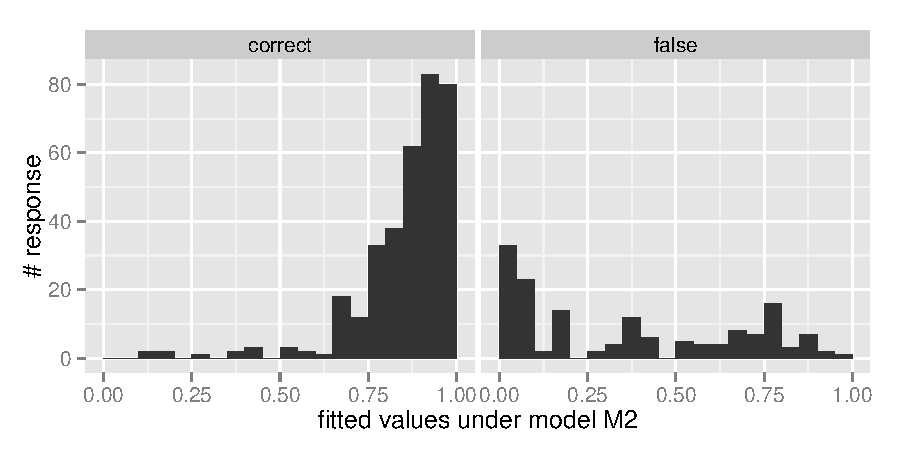
\includegraphics[width=\linewidth]{fitted-m2}
%%\caption{\label{fitted.m2} Histograms of fitted values under model $M2$, facetted by actual performance of participants. On the left, correct responses are shown. The histogram of fitted values is skewed to the right, with most values above 0.5. The histogram on the right corresponds to wrong answers. There are fewer wrong answers, and they tend to have low fitted values, but there are more false positives among them than false negatives for correct answers. }
%%\end{figure}
%
%% xtable(summary(m4)@coefs)
%% latex table generated in R 2.15.1 by xtable 1.7-0 package
%% Fri Oct 12 09:12:32 2012
%\begin{table}[ht]
%\begin{center}
%\begin{tabular}{rrrrrl}
%  \hline
% & Estimate & Std. Error & z value & Pr($>$$|$z$|$) & \\ 
%  \hline  
%$\mu$ & 2.68 & 0.61 & 4.35 & 0.00  & ***\\ [5pt]
%Design\\
%  $d_C$ & 0.00 & -- & -- & -- \\ 
%  $d_H$ & -1.06 & 0.83 & -1.28 & 0.20  \\ 
%  $d_P$ & -0.57 & 0.86 & -0.66 & 0.51 \\ [5pt]
%Questions\\
%  $q_{A1}$ & 0.00 & -- & -- & -- \\ 
%  $q_{A2}$  & -1.85 & 0.74 & -2.50 & 0.01 &* \\ 
%  $q_{A3}$  & -1.11 & 0.77 & -1.44 & 0.15 \\ 
%  $q_{B1}$ & 0.55 & 0.96 & 0.58 & 0.56 \\ 
%  $q_{B2}$  & -1.69 & 0.88 & -1.91 & 0.06 &. \\ 
%  $q_{B3}$  & -1.31 & 0.92 & -1.43 & 0.15 \\ [5pt]
% 
%Interaction \\
%$p_{H, A1}$ &  0.00 & -- & -- & -- \\
%$p_{P,A1}$ &  0.00 & -- & -- & -- \\
%$p_{H, A2}$ &  -3.29 & 1.55 & -2.13 & 0.03 & *\\ 
%$p_{P,A2}$ & -3.03 & 1.33 & -2.28 & 0.02 &*\\ 
%$p_{H,A3}$ &-2.61 & 1.17 & -2.24 & 0.03  & * \\ 
%$p_{P,A3}$ & -2.60 & 1.16 & -2.23 & 0.03 &*\\ 
%$p_{H,B1}$ &-0.26 & 1.21 & -0.22 & 0.83 \\ 
%$p_{P,B1}$ &-0.81 & 1.24 & -0.65 & 0.51 \\ 
%$p_{H,B2}$ & 1.03 & 1.22 & 0.85 & 0.40 \\ 
%$p_{P,B2}$  & -3.48 & 1.63 & -2.14 & 0.03 &*\\ 
%$p_{H,B3}$ & 1.97 & 1.37 & 1.44 & 0.15 \\ 
%$p_{P,B3}$ & -0.62 & 1.26 & -0.50 & 0.62 \\   
%   \hline
%\multicolumn{6}{l}{Signif. codes:  0 `***' 0.001 `**' 0.01 `*' 0.05 `.' 0.1 ` ' 1 }
%\end{tabular}
%\end{center}
%\caption{\label{model2} Model fit for $M2$ measuring correctness of answers in the survey, detailing performance of designs on each question. All design comparisons are with respect to the common angle plot. }
%\end{table}
%

\begin{figure}
\centering 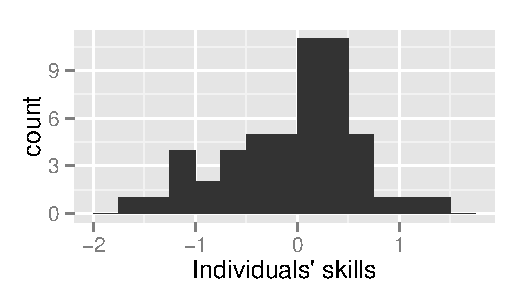
\includegraphics[width=.7\linewidth]{hist-skills}
\caption{\label{skills}Histogram of the predictions of subject-specific skills. }
\vspace{-0.2in}
\end{figure}	
Figure \ref{skills} shows an overview of the predicted skill for each participant under model $M2$. Skills are quite varied between  -1.52 and  1.34, but
a Kolmogorov-Smirnov test  does not show significant deviation from a normal assumption ($p$-value = 0.089).
On the scale of the dependent variable the range in individuals' skills translates to a $17.5 = e^{1.34 - (-1.52)}$ fold increase in the probability of answering a question on the survey correctly between participants with the best skill set and the worst.

In the next section we will investigate the results from the survey in further detail for some questions, and highlight the link to the line width illusion and its inverse.

\subsubsection{Evidence for line width illusions}

Question $A2$ asked participants to order  class levels  according to the number of survivors, fewest to highest. There are 4! = 24 distinct orderings of the levels, corresponding to all permutations of length 4. Some orderings are closer to one another than other orderings.  To quantify distance between each pair of permutations, the Cayley distance is defined as the minimal number of transpositions (i.e. swaps of two elements) necessary to transform one permutation into another.

%The Cayley distance defines a way to quantify the distance between  each pair of permutations; the Cayley distance is defined as the minimal number of transpositions, i.e. swaps of two elements,  necessary to transform one permutation into the other.
This distance is used to define a graph on the space of all permutations: let all permutations be nodes of the graph; for each two permutations with a Cayley distance of one, we add an edge between these nodes to the graph. The resultant regular graph of degree six, i.e. each  node is connected to six other nodes. Between any two nodes, the Cayley distance is then given as length of shortest connecting path shown on the graph.
%The Cayley distance between any two nodes is then given as the length of the shortest connecting path between these two nodes through the graph.
Figure \ref{cubes} shows an overview of the permutation space together with an overview of the survey results. Each permutation is represent by one dot. 

The colored dots on top of the graph correspond to the responses from the survey - the size of the dots is proportional to the number of observers choosing this particular ordering. It becomes obvious from the three graphs in figure \ref{cubes} that
the answers to different designs occupy quite different regions, while answers based  on the same design are quite close --  usually separated by only one edge. 

The correct ordering, as well as the orderings assuming the line width illusion and its reverse are marked with symbols. Answers for the common angle plot are centered around the correct answer, while responses to parallel sets are cluster around the response corresponding to the line width illusion. Due to the small number of responses to the hammock design a clear clustering of the answers is not recognizable, but the answer for the inverse line width illusion is among the responses. Table \ref{a2} gives an overview of all responses to question $A.2$. 

\begin{table}[ht]
\begin{center}
\begin{tabular}{rrrrl}
Order  & CA & H & PS\\
  \hline
  Crew, 1st, 3rd, 2nd &  &  2 &  \\ 
  2nd, 1st, 3rd, Crew &  &  6 &  & inverse illusion \\ 
   Crew, 3rd, 1st, 2nd &  &  1 &  1 \\ 
  2nd, 3rd, 1st, Crew & 1 & 7 & 1 \\ 
  2nd, 3rd, Crew, 1st & 12 &  1 &  2 & correct\\ 
  Crew, 3rd, 2nd, 1st &  2 &  &  \\ 
  3rd, 2nd, Crew, 1st &  1 &  &  \\ 
  1st, 2nd, 3rd, Crew &  1 &  &   \\ 
  1st, 3rd, Crew, 2nd &  1 &  &  2 \\ 
  Crew, 2nd, 3rd, 1st &  &  & 6 &  line width illusion\\  
  1st, 3rd, 2nd, Crew &  &  &  2 \\ 
  2nd, Crew, 3rd, 1st &  &  &  3 \\ 
   \hline
  Total & 18 & 17 & 16 \\ 
   \hline
\end{tabular}
\end{center}
\caption{\label{a2} Responses to question $A.2$: order levels of Class by the number of survivors (smallest to largest). }
\end{table}

%
Common angle plots show the best performance in terms of correctness (66.7\% on 18 responses), compared to a correctness of 11.8\% for parallel sets plots on 16 responses, indicating a significantly better performance of common angle plots at a level of 0.0027, based on a Mantel-Haenszel test (the difference in performance to hammock plots is also significant at a level of 0.0006; but there is no significant difference in correctness between hammock plots and parallel sets.).
While the intuitive assessment of lines by their width orthogonal to their direction is well known, it is surprising to see its strength: in this particular setting, it is strong enough to `shrink' the horizontally widest line for 6 out of 16 participants by at least  44\%, from 212 to below 118, and a further 3 participants perceived the shrinking to below 178, which constitutes a distortion of at least 16\%.

\begin{figure*}
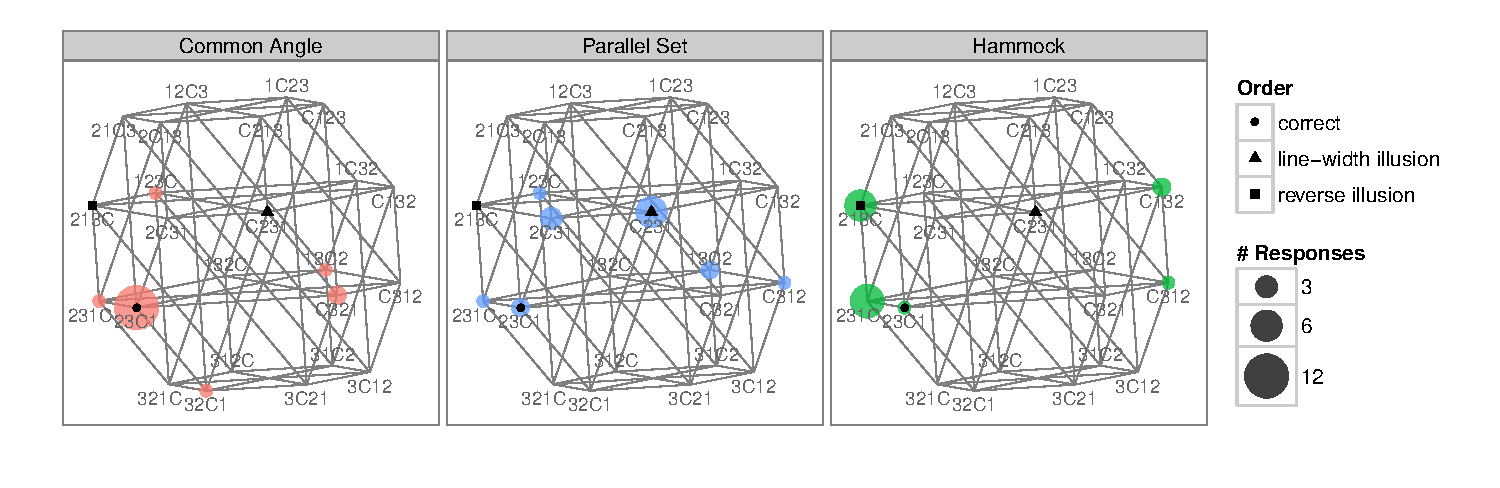
\includegraphics[width=\linewidth]{cubes}
\caption{Answers to question A.2 -- each node corresponds to a single ordering of the levels in variable 'Class'. Lines are drawn between orderings that are only one swap of levels apart. The colored dots show responses from the survey, their sizes depend on the number of responses for each ordering. }
\label{cubes}
\end{figure*}

Responses to question A.3 exhibit a similar pattern, see table \ref{a3}.

\begin{table}[ht]
\begin{center}
\begin{tabular}{rrrrl}
Order & CA & H & PS\\
  \hline
c, b, a &  &  2 &  \\
a, b, c &  1 &  12 &  & inverse illusion\\ 
a, c, b & 13 &  3 &  4 & correct\\ 
b, c, a &  2 &  &  1 \\ 
c, a, b &  2 &  & 9 & line width illusion\\ 
b, a, c &  &  &  2 \\ 
 \hline
  Total & 18 &  17 & 16 \\ 
   \hline
\end{tabular}
\end{center}
\caption{\label{a3}Responses to question A.3: order combinations from smallest to largest, where 'a' is first class female, 'b' are male survivors, and 'c' are crew survivors. }
\end{table}
  
\begin{table}[ht]
\begin{center}
\begin{tabular}{clrrrl}
  Qu & Design & \rotatebox{90}{Correct} & \rotatebox{90}{Incorrect} & \rotatebox{90}{No Answer}   & Reason\\ \hline
  \hline
1 & common &   14 &  2 &   0 \\ 
   & hammock &   15 &  0 &   1 \\ 
 & parallel &   7 &   7 &   0 & line width illusion\\ \hline
2 & common &  16 &   0 &   0 \\ 
& hammock &   9 &   7 &   0 & inverse illusion\\ 
& parallel &  14 &   0 &   0 \\ \hline
3& common &  15 &   1 &   0 \\ 
& hammock &  16 &   0 &   0 \\ 
& parallel &  14 &   0 &   0 \\ 
   \hline
\end{tabular}
\end{center}
\caption{\label{tab:b1}Responses to question set B.1 }
\vspace{-0.25in}
\end{table}


Table \ref{tab:b1} shows a summary to the  three questions of $B.1$ with possible answers ``agree", ``disagree", and ``don't know".
The first two questions are  examples, where the line width illusion, and its reverse will lead to answers that differ from the correct answer. Parallel sets  are susceptible to the line width illusion, while hammock plots suffer from the reverse. The data shows that in about 50\% of the responses we can see this difference. 7 out of 14 answers for the parallel sets plots in question 1 deviate from the correct answer, and 7 out of 16 responses corresponding to hammock plots in question 2 show the wrong answer.


\subsubsection{Opinion on common angle plots}
Answers to the question of `which chart did you like better?' are shown in table \ref{tab:prefer}. There is a pretty clear endorsement in favor of common angle plots versus the other two types of displays.
Asked for a reason for their preference over parallel sets, 8 participants cited a facilitated comparison of width, area or ``size", 3 saw the common angle plots as preferable, and the remaining answers related to a 'more logical' structure or generally 'easier' choice.
Reasons for not preferring common angle plots boiled down to a preference for straight lines. This purely aesthetic preference is deeply rooted and in our opinion the biggest challenge for common angle plots.
% latex table generated in R 2.15.1 by xtable 1.7-0 package
% Wed Oct 31 10:28:55 2012
\begin{table}[ht]
\begin{center}
\begin{tabular}{cccrrr}
  \hline
&\multicolumn{5}{r}{Which chart did you like better?}\\
&&& Chart 1 &  Chart 2 \\ 
  \hline
  PS &vs&  {\bf CA} & 2 & \bf 6 \\ 
 {\bf  CA} & vs &  PS & \bf 4 & 2 \\ 
  H & vs &   {\bf  CA} & 3 & \bf 5 \\ 
   {\bf  CA} & vs &  H & \bf 8 & 2 \\ 
  H & vs &  PS & 3 & 5 \\ 
  PS & vs &  H & 1 & 5 \\ 
   \hline
\end{tabular}
\caption{\label{tab:prefer} Preferences for first or second chart across all six combinations of questions and chart types. }
\vspace{-0.3in}
\end{center}
\end{table}

\section{Conclusion}
The conclusion goes here.





% if have a single appendix:
%\appendix[Proof of the Zonklar Equations]
% or
%\appendix  % for no appendix heading
% do not use \section anymore after \appendix, only \section*
% is possibly needed

% use appendices with more than one appendix
% then use \section to start each appendix
% you must declare a \section before using any
% \subsection or using \label (\appendices by itself
% starts a section numbered zero.)
%


\appendices
%\section{Proof of the First Zonklar Equation}
%Appendix one text goes here.
%
%% you can choose not to have a title for an appendix
%% if you want by leaving the argument blank
%\section{}
%Appendix two text goes here.


% use section* for acknowledgement
\section*{Acknowledgment}


The survey for this study was carried out with approval from  IRB-ID 12-204.


% Can use something like this to put references on a page
% by themselves when using endfloat and the captionsoff option.
\ifCLASSOPTIONcaptionsoff
  \newpage
\fi



% trigger a \newpage just before the given reference
% number - used to balance the columns on the last page
% adjust value as needed - may need to be readjusted if
% the document is modified later
%\IEEEtriggeratref{8}
% The "triggered" command can be changed if desired:
%\IEEEtriggercmd{\enlargethispage{-5in}}

\appendices
%\section{Proof of the First Zonklar Equation}
Appendix one text goes here.

% you can choose not to have a title for an appendix
% if you want by leaving the argument blank
	%\section{}
	%Appendix two text goes here.Appendix two text goes here.Appendix two text goes here.Appendix two text goes here.Appendix two text goes here.Appendix two text goes here.Appendix two text goes here.Appendix two text goes here.Appendix two text goes here.Appendix two text goes here.Appendix two text goes here.Appendix two text goes here.Appendix two text goes here.Appendix two text goes here.Appendix two text goes here.Appendix two text goes here.Appendix two text goes here.Appendix two text goes here.Appendix two text goes here.Appendix two text goes here.Appendix two text goes here.Appendix two text goes here.Appendix two text goes here.Appendix two text goes here.Appendix two text goes here.
	%

% use section* for acknowledgement
\ifCLASSOPTIONcompsoc
  % The Computer Society usually uses the plural form
%  \section*{Acknowledgments}
\else
  % regular IEEE prefers the singular form
%  \section*{Acknowledgment}
\fi


%The authors would like to thank...The authors would like to thank...The authors would like to thank...The authors would like to thank...The authors would like to thank...The authors would like to thank...The authors would like to thank...The authors would like to thank...The authors would like to thank...The authors would like to thank...The authors would like to thank...The authors would like to thank...The authors would like to thank...


% Can use something like this to put references on a page
% by themselves when using endfloat and the captionsoff option.
\ifCLASSOPTIONcaptionsoff
  \newpage
\fi


% trigger a \newpage just before the given reference
% number - used to balance the columns on the last page
% adjust value as needed - may need to be readjusted if
% the document is modified later
%\IEEEtriggeratref{8}
% The "triggered" command can be changed if desired:
%\IEEEtriggercmd{\enlargethispage{-5in}}

% references section

% can use a bibliography generated by BibTeX as a .bbl file
% BibTeX documentation can be easily obtained at:
% http://www.ctan.org/tex-archive/biblio/bibtex/contrib/doc/
% The IEEEtran BibTeX style support page is at:
% http://www.michaelshell.org/tex/ieeetran/bibtex/
\bibliographystyle{IEEEtran}
% argument is your BibTeX string definitions and bibliography database(s)
\bibliography{references}
%
% <OR> manually copy in the resultant .bbl file
% set second argument of \begin to the number of references
% (used to reserve space for the reference number labels box)
%\begin{thebibliography}{1}
%
%\bibitem{IEEEhowto:kopka}
%%This is an example of a book reference
%%H. Kopka and P.W. Daly, \emph{A Guide to {\LaTeX}}, third ed. Harlow, U.K.: Addison-Wesley, 1999.
%
%
%%This is an example of a Transactions article reference
%%D.S. Coming and O.G. Staadt, "Velocity-Aligned Discrete Oriented Polytopes for Dynamic Collision Detection," IEEE Trans. Visualization and Computer Graphics, vol.�14,� no.�1,� pp. 1-12,� Jan/Feb� 2008, doi:10.1109/TVCG.2007.70405.
%
%%This is an example of a article from a conference proceeding
%%H. Goto, Y. Hasegawa, and M. Tanaka, "Efficient Scheduling Focusing on the Duality of MPL Representation," Proc. IEEE Symp. Computational Intelligence in Scheduling (SCIS '07), pp. 57-64, Apr. 2007, doi:10.1109/SCIS.2007.367670.
%
%%This is an example of a PrePrint reference
%%J.M.P. Martinez, R.B. Llavori, M.J.A. Cabo, and T.B. Pedersen, "Integrating Data Warehouses with Web Data: A Survey," IEEE Trans. Knowledge and Data Eng., preprint, 21 Dec. 2007, doi:10.1109/TKDE.2007.190746.
%
%%Again, see the IEEEtrans_HOWTO.pdf for several more bibliographical examples. Also, more style examples
%%can be seen at http://www.computer.org/author/style/transref.htm
%\end{thebibliography}

% biography section
% 
% If you have an EPS/PDF photo (graphicx package needed) extra braces are
% needed around the contents of the optional argument to biography to prevent
% the LaTeX parser from getting confused when it sees the complicated
% \includegraphics command within an optional argument. (You could create
% your own custom macro containing the \includegraphics command to make things
% simpler here.)
%\begin{biography}[{\includegraphics[width=1in,height=1.25in,clip,keepaspectratio]{mshell}}]{Michael Shell}
% or if you just want to reserve
\begin{IEEEbiographynophoto}{Heike Hofmann}
is an associate professor of Statistics at Iowa State University. She is a member of the inter-disciplinary Human Computer Interaction program at Iowa State and serves as faculty member for the Bioinformatics and Computational Biology program. Her research interests are the visual exploration of high-dimensional and large data. Her research group has been the recipient of several awards for their data detective and visualization skills.  
\end{IEEEbiographynophoto}
\vspace{-.25in}
\begin{IEEEbiographynophoto}{Marie Vendettuoli}
is a graduate student at Iowa State University, with majors in Human Computer Interaction and Bioinfomatics \& Computational Biology. She is a past IGERT Fellow and currently interns with the Statistics section at USDA. Her research interests involve the use of interactive visualizations in exploratory data analysis.
\end{IEEEbiographynophoto}

% You can push biographies down or up by placing
% a \vfill before or after them. The appropriate
% use of \vfill depends on what kind of text is
% on the last page and whether or not the columns
% are being equalized.

%\vfill

% Can be used to pull up biographies so that the bottom of the last one
% is flush with the other column.
%\enlargethispage{-5in}



% that's all folks
\end{document}



